%%%% Modèle proposé par henry.costedoat@universite-paris-saclay.fr %%%%
%%%% Grand fan de LaTeX %%%%
%%%% Inspiré par un modèle proposé par frederic.mazaleyrat@ens-paris-saclay.fr 

%%%% 4 fevrier 2022  %%%%

\documentclass[english,13pt,a4paper]{article}
\usepackage[T1]{fontenc}
\usepackage[english]{babel}
\usepackage{amsmath}
\usepackage{amsfonts}
%\usepackage{fancyhdr}
\usepackage{amssymb}
\usepackage{xcolor} % où xcolor selon l'installation
\definecolor{BleuFonce}{RGB}{0,74,117}
\usepackage[framemethod=tikz]{mdframed}
\usepackage{multirow} %% Pour mettre un texte sur plusieurs rangées
\usepackage{multicol} %% Pour mettre un texte sur plusieurs colonnes
\usepackage{tikz}
%\usepackage{graphicx}
%\usepackage[absolute]{textpos} 
%\usepackage{colortbl}
\usepackage{array}
\usepackage{geometry}
\usepackage{hyperref}
\usepackage{float}
%\usepackage{floatrow}
%\usepackage{bashful}% pour gérer le scripting bash
\usepackage{listing}
%\usepackage{fullpage}
\usepackage{caption}
\usepackage{subcaption}
\usepackage{lipsum}
%\usepackage{wasysym}
\usepackage{amsthm}
\usepackage{mathrsfs}
\usepackage{mathtools}
\usepackage{stmaryrd}
\usepackage{enumitem}
\usepackage{xfrac}
\usepackage{dsfont}
\usepackage{comment}
%\usepackage{hhline}
%\usepackage{scrextend}
%\usepackage{keyval}
%\usepackage{filecontents}
\usepackage{pict2e}
\usepackage{algorithm}
\usepackage{algpseudocode}

%\usepackage{parskip}
%\usepackage[thinlines]{easytable}


%---------- BIBLIO ----------%
\usepackage[backend=biber,style=alphabetic,sorting=ynt]{biblatex}
\addbibresource{biblio.bib} % import the bibliography file
\addto{\captionsenglish}{\renewcommand{\bibname}{\textsc{References}}}


%---------- For big table of contents ----------%
\usepackage{tocloft}

\renewcommand{\cfttoctitlefont}{\Huge\bfseries}% Similar to \chapter* in report
\setlength{\cftbeforetoctitleskip}{50pt}% Similar to \chapter* in report
\setlength{\cftaftertoctitleskip}{40pt}% Similar to \chapter* in report
\addtolength{\cftsecnumwidth}{10pt}
%-----------------------------------------------%

\geometry{margin=2cm}

\graphicspath{{./Images/}}


%\renewcommand{\familydefault}{<font family>} % pour changer la police voir : https://latex-tutorial.com/changing-font-style/

\algnewcommand\algorithmicvar{\textbf{Variables:}}
\algnewcommand\Var{\item[\algorithmicvar]}


\theoremstyle{definition}
\newtheorem{theorem}{Theorem}[section]
\newtheorem{proposition}{Proposition}[section]
\newtheorem{corollary}{Corollary}[section]
\newtheorem*{example}{Example}
%\newtheorem{definition}{Definition}[section]
\newtheorem{lemma}{Lemma}[section]

\theoremstyle{remark}
\newtheorem*{remark}{Remark}
\newtheorem*{reminder}{Reminder}

% \renewenvironment{definition}
%   {\par\noindent\normalfont\textbf{Definition \thedefinition}\par\nopagebreak%
%   \begin{mdframed}[
%      linewidth=1pt,
%      linecolor=black,
%      bottomline=false,topline=false,rightline=false,
%      innerrightmargin=0pt,innertopmargin=0pt,innerbottommargin=0pt,
%      innerleftmargin=1em,% Distance between vertical rule & proof content
%      skipabove=.5\baselineskip
%    ]}
%   {\end{mdframed}}



\newtheoremstyle{defstyle}% Custom theorem style
  {3pt}% Space above
  {3pt}% Space below
  {}% Body font
  {}% Indent amount
  {\bfseries}% Theorem head font
  {.}% Punctuation after theorem head
  {.5em}% Space after theorem head
  {%
    \thmname{#1}% Name of theorem
    \thmnumber{ #2}% Number of theorem
    \thmnote{ (#3)}% Optional note
  }

\theoremstyle{defstyle}
\newtheorem{definition}{Definition}[section]

\renewenvironment{definition}[1][]{
    \refstepcounter{definition}% Increment the definition counter
    \par\noindent\textbf{Definition \thedefinition}%
    \if\relax\detokenize{#1}\relax\else~(#1)\fi\par\nopagebreak%
    \begin{mdframed}[
        linewidth=.8pt,
        linecolor=darkgray,
        bottomline=false,
        topline=false,
        rightline=false,
        innerrightmargin=0pt,
        innertopmargin=0pt,
        innerbottommargin=0pt,
        innerleftmargin=1em,% Distance between vertical rule & definition content
        skipabove=.5\baselineskip
    ]}
    {\end{mdframed}}


\renewenvironment{example}[1][]{
    %{\refstepcounter{definition}% Increment the definition counter
    \par\noindent\textbf{Example.}%
    %\if\relax\detokenize{#1}\relax\else~(#1)\fi\par\nopagebreak%
    \begin{mdframed}[
        linewidth=.8pt,
        linecolor=darkgray,
        bottomline=false,
        topline=false,
        rightline=false,
        innerrightmargin=0pt,
        innertopmargin=0pt,
        innerbottommargin=0pt,
        innerleftmargin=1em,% Distance between vertical rule & definition content
        skipabove=.5\baselineskip
    ]}
    {\end{mdframed}}

\newcommand{\I}[1]{\mathbb{#1}}
\DeclareMathOperator{\sgn}{sgn}
\renewcommand{\epsilon}{\varepsilon}
\renewcommand{\emptyset}{\varnothing}


%-------- Section Numbering -------%
\renewcommand*{\thesection}{\Roman{section}.}
\renewcommand*{\thesubsection}{\Roman{section}.\arabic{subsection}}





\begin{document}

\begin{titlepage}

%\thispagestyle{empty}

\newgeometry{left=6cm,bottom=0.5cm, top=0.25cm, right=1cm}

\tikz[remember picture,overlay] \node[opacity=1,inner sep=0pt] at (2.2mm,-165mm){
\includegraphics{Fond1.png}}; % Fond changeable 

% fonte sans empattement pour la page de titre
\fontfamily{fvs}\fontseries{m}\selectfont

\color{white}

 
%**************************************************************
%********************  LOGO  DE  POLYTECH  ********************
%****** CHANGER L'IMAGE POUR UN AUTRE POLYTECH QUE SACLAY *****
%* VOIR LES LOGOS DISPONIBLES, ET REMPLACER LE NOM CI-DESSOUS *
%**************************************************************

\vspace{-5mm} % à ajuster en fonction de la hauteur du logo
               % décalera le texte en dessous
\flushright 
\includegraphics[width=70mm]{logo-ULB.jpg} % nom du logo du polytech

\vspace{-23mm}

\flushleft 
\includegraphics[height=19mm]{Images/VUB_RGB.png} %\caption{cghj}




%*****************************************************
%******************** TITRE **************************
%*****************************************************
\flushright
\vspace{15mm} % à régler éventuellement
\color{BleuFonce}
\fontfamily{cmss}\fontseries{m}\fontsize{22}{26}\selectfont
Review of `Comparing sequences without using alignments: application to
HIV/SIV subtyping'

\normalsize
\color{black}
%*****************************************************

%\fontfamily{fvs}\fontseries{m}\fontsize{8}{12}\selectfont

\vspace{1.5cm}
\normalsize

\textbf{Supervised by Prof. Mathieu Defrance (\textit{Machine Learning Group - ULB}) \\ \& Prof. Wim Vranken (\textit{Bioengineering Sciences Department - VUB})}

\vspace{15mm}

Master's in Computer Science\\  %% nom spécialité / enseignement

\vspace{15mm}

\Large 
{\color{BleuFonce} \textbf{Tom\'as GUIJA VALIENTE}}\\
{\color{BleuFonce} \textbf{Benjamin OBERTHÜR}}

\vspace{20mm}

\centering

\hrule
\begin{abstract}
    This article presents a review of an innovative method for alignment-free sequence comparison in the field of bioinformatics. The method, introduced in a relatively early published article, enables the identification of evolutionary relationships between sequences and highlights divisions into subtypes. Despite the absence of a description for the cluster merging method in the original article, the remaining parts of the algorithm were successfully re-implemented, demonstrating that the experiments were not environment-dependent and consistently produced reliable results. Furthermore, comparisons with more recent methods were discussed, acknowledging the possibility of newer approaches offering improved efficiency, runtime, and accuracy.\\

    The review emphasizes the significance of the alignment-free sequence comparison approach, particularly in addressing challenges posed by sequence alterations and the limitations of classic alignment methods. By leveraging the concept of $N$-words (or k-mers in today's scientific literature), dissimilarity matrices and clustering trees were constructed, providing insights into the evolutionary relationships among the sequences.\\

    The article concludes by highlighting the potential of the reviewed method as a valuable tool in phylogenetic analysis. It suggests avenues for further research, including exploring alternative clustering techniques and investigating the impact of various distance measures for enhanced accuracy. Overall, this review contributes to the understanding of alignment-free sequence comparison methods and their applications in studying evolutionary relationships among biological sequences.
\end{abstract}
\vspace*{3mm}
\hrule

\end{titlepage}

%%%%%%%%%%%%%%%%%%%%%%%%%%%%%%%%%%%%%%%%%%%%%%%%%%%%%%%%%%%%%%

\normalsize
\tableofcontents

\newpage

\section{Introduction and summary of the article}\label{seq:summary}

This article describes the problem in sequence comparison, which arises when attempting to compare a large number of sequences together. Classic sequence alignment methods often struggle to effectively handle certain types of sequence alterations, such as insertions or deletions. Intuitive approaches to address this problem without alignment involve examining the frequency of nucleotides or amino acids. However, this method lacks meaningfulness, as sequences with similar frequencies can still exhibit significant differences. A more sophisticated and effective approach is dealing with what~\cite{didier_comparing_2007} calls $N$-words. With those, we can compute dissimilarities between sequences~\cite{karlin1994comparisons} which can help us show evolutionary relationships between sequences.\\

\subsection{Local decoding method of order $N$}

The first step of this analysis presented by~\cite{didier_comparing_2007} is the local decoding method of order $N$, or $N$-local decoding. \\

\begin{definition}[$N$-words]\label{def:nword}
    In a sequence, an $N$-word is a \textbf{contiguous sub-sequence of size $N$} within the given sequence. The set of $N$-words for a sequence consists of all its sub-sequences of size $N$.
\end{definition}

\begin{example}
    The set of the 3-words of the sequence $AGTACGT$ is $AGT$, $GTA$, $TAC$, $ACG$, $CGT$.
\end{example}

\vspace{3mm}

Let $S = S_1 S_2 \ldots S_i \ldots S_{|S|}$ be a sequence, where $i$ denotes a site (or index) within $S$. For a given $N \in \I N^*$, we consider the set of $N$-words of $S$ covering the site $i$.\\


\begin{definition}[Direct relation]\label{def:direct_rel}
    Two sites are said \textbf{directly related} if they have the same position in two (or more) occurences of the same $N$-word.
\end{definition}

\begin{example}
    (We take the example on Figure 6a in~\cite{didier_comparing_2007}). Let seq1 = CATTG T{\color{red} CCGC \textbf{T}GGAC} CACAC and seq2 = {\color{red} CACT\textbf{T} GGAC}A CATAC CATGC. We consider the site 11 in seq1 and the site 5 in seq2 (bolded in their definitions), and look at the 5-words covering this site (contained in the sites colored in red).\\

    \begin{minipage}{.47\textwidth}
        \begin{tabular}{*4c | c | *4c}
            \cline{5-5}
            C & C & G & C & \textbf{T} & G & G & A & C \\
            \hline
            C & C & G & C & T &   &   &   &  \\
              & C & G & C & T & G &   &   &  \\
              &   & G & C & T & G & G &   &  \\
              &   &   & C & T & G & G & A &  \\
              &   &   &   & \textbf{T} & \textbf{G} & \textbf{G} & \textbf{A} & \textbf{C} \\
            \cline{5-5}
        \end{tabular}
    \end{minipage}
    \begin{minipage}{.47\textwidth}
        \begin{tabular}{*4c | c | *4c}
            \cline{5-5}
            C & A & C & T & \textbf{T} & G & G & A & C \\
            \hline
            C & A & C & T & T &   &   &   &  \\
              & A & C & T & T & G &   &   &  \\
              &   & C & T & T & G & G &   &  \\
              &   &   & T & T & G & G & A &  \\
              &   &   &   & \textbf{T} & \textbf{G} & \textbf{G} & \textbf{A} & \textbf{C} \\
            \cline{5-5}
        \end{tabular}
    \end{minipage}

    \noindent
    The 5-word TGGAC appears in both these sequences, and the sites 11 in seq1 and 5 in seq2 are both in first position of the 5-word, so these two sites are \textbf{directly related}
\end{example}

\begin{definition}[Transitivity and transitive closure]
    Let $\mathcal{R}$ and $\mathcal{R}'$ be binary relations. $\mathcal{R}$ is said to be \textbf{transitive} if it respects the following property~\cite{cauchy1821cours}:
    \[
        a \mathcal{R} b \land b \mathcal{R} c \implies a \mathcal{R} c 
    \]
    $\mathcal{R}'$ is the \textbf{transitive closure} of $\mathcal{R}$ if~\cite{schroder1877operationskreis}:
    \[
        \forall a, \, b; \; a \mathcal{R} b \implies a \mathcal{R'} b
    \]
    and
    \[
        \forall a, \, b, \, c; \; a \mathcal{R} b \land b \mathcal{R} c \implies a \mathcal{R'} c
    \]
\end{definition}

\begin{definition}
    We define the (simple) relation between two sites as the transitive closure of the direct relation. Therefore, we say that two sites are related if there is a (finite) chain of direct relations linking those sites.
\end{definition}

These related sites can be categorized into distinct equivalence classes, as the relation we described satisfies the properties of an equivalence relation, namely, reflexivity, symmetry, and transitivity.~\cite{didier_comparing_2007} refers to these equivalence classes as $N$-classes.

\begin{definition}[$N$-classes]
    An $N$-class can be defined as follows,with $a$ being the identifier of the $N$-class:
    \[
        C(a) = \{x \in \llbracket 1, \, |S| \rrbracket\footnotemark; \; x \text{ is related with } a\}
    \]
\end{definition}
\footnotetext{$\llbracket \cdot, \, \cdot \rrbracket \: : \: \I N \times \I N \to \I N$: Integer interval, $\llbracket a, \, b \rrbracket = \{a, \, a+1, \, \ldots, \, b\}$}

Consequently, by assigning a unique identifier to each $N$-class, we can rename every site in the entire sequence by appending the nucleotide (or amino acid) with the identifier of the class to which it belongs. However, there may exist sites that are not related to any other site in any other sequence, resulting in singleton $N$-classes. To avoid excessive and unnecessary identifiers, which could lead to unreadable representations, we represent these sites solely by their nucleotide or amino acid.


\subsection{Dissimilarity matrix and clustering tree}\label{sseq:dissim}

Now that we have our new sequences divided into disjoint $N$-classes of sites, we aim to compare each sequence. To achieve that, we need to select a measure of (dis-)similarity.~\cite{didier_comparing_2007} chose the one defined in~\cite{didier2006decoding}.\\

Let's introduce the following notation. $|s|_x$ is the number of occurences of the identifier $x$ in the sequence $s$. For each pair of sequence and identifier $(s, \, x)$, we compute the value of $|s|_x$.

\begin{example}
    We consider the following rewriten sequences:\\

    \begin{table}[H]
        \centering
        \begin{tabular}{r|l}
            seq1 & $C \, A \, T_0 \, T_1 \, G_0 \, T_2 \, C_0 \, C_1 \, G \, C_2 \, T_3 \, G_1 \, G_2 \, A_0 \, C_3 \, C_4 \, A \, C \, A \, C \, C \, T_0 \, T_1 \, G_0 \, T_2 \, C_0 \, C_1 \, C \, T \, A$\\

            seq2 & $C_5 \, A_1 \, C_6 \, T_4 \, T_3 \, G_1 \, G_2 \, A_0 \, C_3 \, A \, C \, A \, T \, A \, C \, C \, A \, T \, G \, C$\\

            seq3 & $C_5 \, A_1 \, C_6 \, T_4 \, T_3 \, C \, T \, T \, T \, C \, C_2 \, T_3 \, G_1 \, G_2 \, A_0 \, C_3 \, C_4 \, T \, C \, C$
        \end{tabular}
        \caption{Rewriten sequence (picked from~\cite{didier_comparing_2007})}
    \end{table}

    \begin{table}[H]
        \centering
        \begin{tabular}{|*4{c|}}
            \hline
                  & seq1 & seq2 & seq3\\
            \hline
            $A_0$ &  1   &  1   &  1  \\
            $A_1$ &  0   &  1   &  1  \\
            $T_0$ &  2   &  0   &  0  \\
            $T_1$ &  2   &  0   &  0  \\
            $T_2$ &  2   &  0   &  0  \\
            $T_3$ &  1   &  1   &  2  \\
            $T_4$ &  0   &  1   &  1  \\
            $C_0$ &  2   &  0   &  0  \\
            $C_1$ &  2   &  0   &  0  \\
            $C_2$ &  1   &  0   &  1  \\
            $C_3$ &  1   &  1   &  1  \\
            $C_4$ &  1   &  0   &  1  \\
            $C_5$ &  0   &  1   &  1  \\
            $C_6$ &  0   &  1   &  1  \\
            $G_0$ &  2   &  0   &  0  \\
            $G_1$ &  1   &  1   &  1  \\
            $G_2$ &  1   &  1   &  1  \\
            \hline
        \end{tabular}
        \caption{Count of each identified site in each sequence}
    \end{table}
\end{example}

Then to compute the similarity between each sequences, we apply the following formula:
\[
    \text{sim}(\text{seq}, \, \text{seq}') = \frac{\sum_x \min(|\text{seq}|_x, \, |\text{seq}'|_x)}{\min(|\text{seq}|, \, |\text{seq}'|)}
\]

\begin{example}
    for $i, \, j \in \{\text{seq1}, \, \text{seq2}, \, \text{seq3}\}$:
    \[
        \text{Sim} = {(\text{sim}(i, \, j))}_{i<j} =
        \begin{pmatrix}
            - & \frac{5}{20} & \frac{7}{20} \\
               & - & \frac{9}{20} \\
               &    & -
        \end{pmatrix}
        =
        \begin{pmatrix}
            - & 0.25 & 0.35 \\
               & - & 0.45 \\
               &    & -
        \end{pmatrix}
    \]
\end{example}

The dissimilarity (or distance) can easily be obtained by taking the complement to 1 of the similarity.\\

Now that we have our mesure of distance between sequences, we can perform an agglomerative hierarchical clustering~\cite{anderberg1973cluster} that can give us an idea of a potential mutative evolution of HIV and SIV, that can be interpreted as subtypes of these viruses. However, in order to perform this clustering, we need a method to compute the distance between clusters containing multiple sequences. The article does not present one, so we had to design our own, described in Subsection~\ref{ssec:merge} 


\subsection{Bootstrapping}

Finally, in order to have more confidence in the results, the authors use the statistical technique of `bootstrapping'~\cite{efron1979bootstrap}. In the case of sequence comparison, the method proposed in~\cite{felsenstein1980confidence} was considered and adapted to local decoded sequences. The motivation behind using this method is that the results obtained may possess a certain degree of uncertainty due to data limitations or noise.\\

For each sequence in the original data, a random replicate of the same size is created by randomly selecting sites from the original data with replacement and concatenating them. Once these artificial sets have been generated, the same analysis performed on the original set is carried out on the new set. By comparing the results obtained from the original set with those from the artificial sets, the stability of the method can be assessed, taking into account the inherent uncertainty introduced by the data.

\section{Material \& Method}\label{sec:mat_method}

\subsection{Data Sets}\label{ssec:DS}

We used two different sequence sets to run our experiments: one given from Gilles Didier, co-author of~\cite{didier_comparing_2007}, and another that we retrieved ourselves, both coming from the data base maintened by the `Los Alamos National Laboratory'\footnote{\url{https://www.hiv.lanl.gov}}. The first set contains 66 sequences writen prior to 2007~\footnote{The sequences presented in figure 1 of~\cite{didier_comparing_2007}, with 4 missing sequences}, and the second one has been created from the query to have 50 sequences sampled in 2016 in Germany (so that we look at mutations in a restrained place and time).

\subsection{Cluster merging method}\label{ssec:merge}

For our cluster merging method, we drew inspiration from centroid linkage methods~\cite{duda1973pattern}. When considering a cluster $\mathcal{C}$ containing more than one sequence, we create an artificial sequence with a length equal to that of the shortest sequence within the cluster. This artificial sequence is defined as follows:
\[
    \widetilde{\text{seq}}_i = \arg \max_{s_i; \,s \in \mathcal C} \frac{s_i}{|\mathcal C|},  \quad \forall i \in \llbracket 1, \, n \rrbracket, \, n = \min_{s \in \mathcal{C}} |s| 
\]
In simpler terms, for each site of the artificial sequence, we select the $N$-class that appears most frequently at the corresponding site across the different sequences in the cluster. If multiple $N$-classes have the same frequency of occurrence, we choose the first element with the highest frequency. To compute the distance between two clusters, we utilize the same formula as shown in Subsection~\ref{sseq:dissim}. 



\section{Experiments and Results}

\subsection{Original set of sequence}

\subsubsection{Comparison of the clustering trees}

We have followed the procedure outlined in the summary (Section~\ref{seq:summary}) and used the same length of $N$-words as in the article, i.e. $N=15$. The resulting dissimilarity matrix for the set of sequences can be found at the following path: \texttt{data/Dissimilarity Matrices/dissmatrix\_\_66\_sequences.txt} within the repository. Since the matrix is too large to be displayed here, please refer to the file for its contents. Additionally, the corresponding cluster tree for this dissimilarity matrix is presented in Figure~\ref{fig:tree66} in the Appendix. It follows the cluster tree from the original article, which can be found in Figure~\ref{fig:original_tree66}.\\

When looking at both the figures, we can see that they are very alike. Let's take the following sequences in example, that both come from the smaller `block' of each tree:

\begin{figure}[H]
    \centering
    \begin{subfigure}{.48\textwidth}
        \centering
        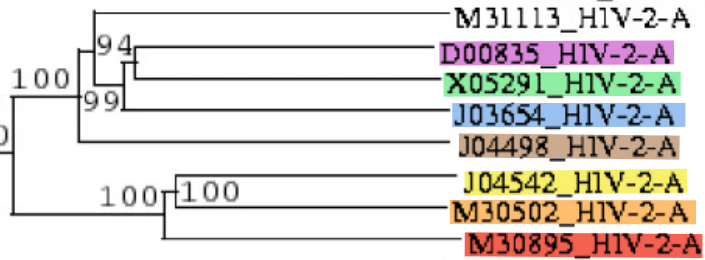
\includegraphics[width=\textwidth]{Images/Example2_Orig66.png}
        \caption{Part of the original tree}
    \end{subfigure}
    \hfill
    \begin{subfigure}{.48\textwidth}
        \centering
        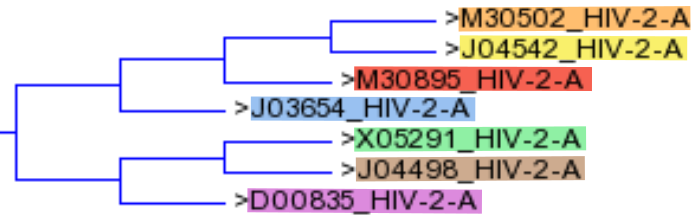
\includegraphics[width=\textwidth]{Images/Example2_66.png}
        \caption{Part of the generated tree}
    \end{subfigure}
\end{figure}

On these parts of the trees, we can see that there is a large resemblance between the two. The few differences between the two are permutations between the subtrees (\texttt{J03654} that should be in the other subtree and \texttt{D00835} that should be deeper in the subtree), and the sequence \texttt{M31113} that do not appear in the generated tree, as it is alone as child of the root node. This change can be one of the possibly significant change between the two trees\\

We can look at a second example:

\begin{figure}[H]
    \centering
    \begin{subfigure}{0.48\textwidth}
        \centering
        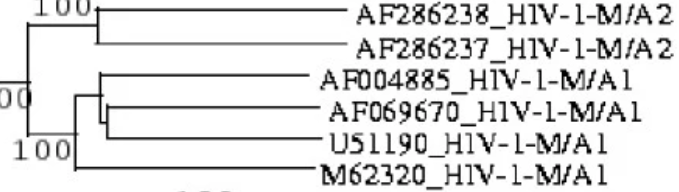
\includegraphics[width=\textwidth]{Images/Example_Orig66.png}
        \caption{Another part of the original tree}
    \end{subfigure}
    \hfill
    \begin{subfigure}{0.48\textwidth}
        \centering
        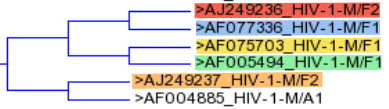
\includegraphics[width=\textwidth]{Images/Example_66.png}
        \caption{Another part of the generated tree}
    \end{subfigure}
\end{figure}

There are more difference between these two parts, but still pretty small. \texttt{AF005494} should take \texttt{AJ249236}'s place, and the latter become a sibling of \texttt{AJ249237}, with the additional (non-colored) sequences that should come or leave the subtree 

\subsubsection{Bootstrapping}

We conducted 10 different bootstraps to assess the reliability of our method. The resulting trees can be found at the following path: \texttt{data/Tree visualization/Bootstraps\_66\_sequences}. All the trees exhibit the same overall structure, with three distinct blocks of sequences that remain separate from each other. Additionally, the sequence \texttt{M31113} consistently maintains the same position in all the bootstrap trees. However, some permutations between sequences within the different blocks can still be observed. These permutations tend to occur in the deeper half of the tree for the ``large block''.\\

While the bootstrap trees are not identical to each other or to the original generated tree in terms of their structure, our method still accurately distinguishes between the subtypes of HIV and SIV. All the sequences of subtypes HIV-1-M are grouped together in the larger subtree, and the sequences of subtype HIV-2-A in another subtree. This indicates the robustness of our approach, despite variations in the specific arrangements of the trees and permutations within the sequence blocks.


\subsection{`German' set of sequences}

In Figure~\ref{fig:tree50}, we can remark that the various subtypes of HIV are well-clustered within the clustering tree. Notably, the four sequences belonging to subtype 01AE are grouped together, as are the sequences of subtype B. However, the sequences of subtype C display a slight scattering pattern in the tree. A majority of the subtype C sequences are clustered near the top of the tree, with one sequence positioned slightly higher, and the remaining sequences forming another subtree within the tree.\\

Based on the observations made for the previous set of sequences, it is worth noting that the bootstraps for the current set - located at \texttt{Trees/Bootstraps\_50\_sequences} in the repository - exhibit a consistent structure. Furthermore, only minimal permutations among the leaf nodes are observed across the different bootstraps. Considering the previous paragraph, it can be concluded that our algorithm demonstrates a high level of reliability for this particular dataset as well.

\section{Conclusion}

In this review, we have observed an innovative method (considering the relatively early publishing year of the article) for alignment-free sequence comparison. This method enables the identification of evolutionary relationships between sequences and highlights divisions into subtypes.\\

Although the cluster merging method was not described in the article, we were able to re-implement the remaining parts of the described algorithm. This allowed us to demonstrate that the experiments were not environment-dependent, and we obtained consistent results. Additionally, we confirmed the effectiveness and reliability of our cluster merging method.\\

As mentioned earlier, this article was published in 2007, and since then, other methods may have been developed with better efficiency, runtime, and correctness. This is likely the case with the SeqDistK method~\cite{Liu2021seqdistk}. This method uses the same algorithmic pattern as the article under review but employs seven different $k$-mer (or $N$-word) distances. It also utilizes the Unweighted Pair Group Method with Arithmetic Mean algorithm~\cite{sokal1975statistical} to construct the tree.


\vfill

\addcontentsline{toc}{section}{References}
\printbibliography

\addcontentsline{toc}{section}{Appendix}
\section*{Appendix}

\begin{figure}[H]
    \centering
    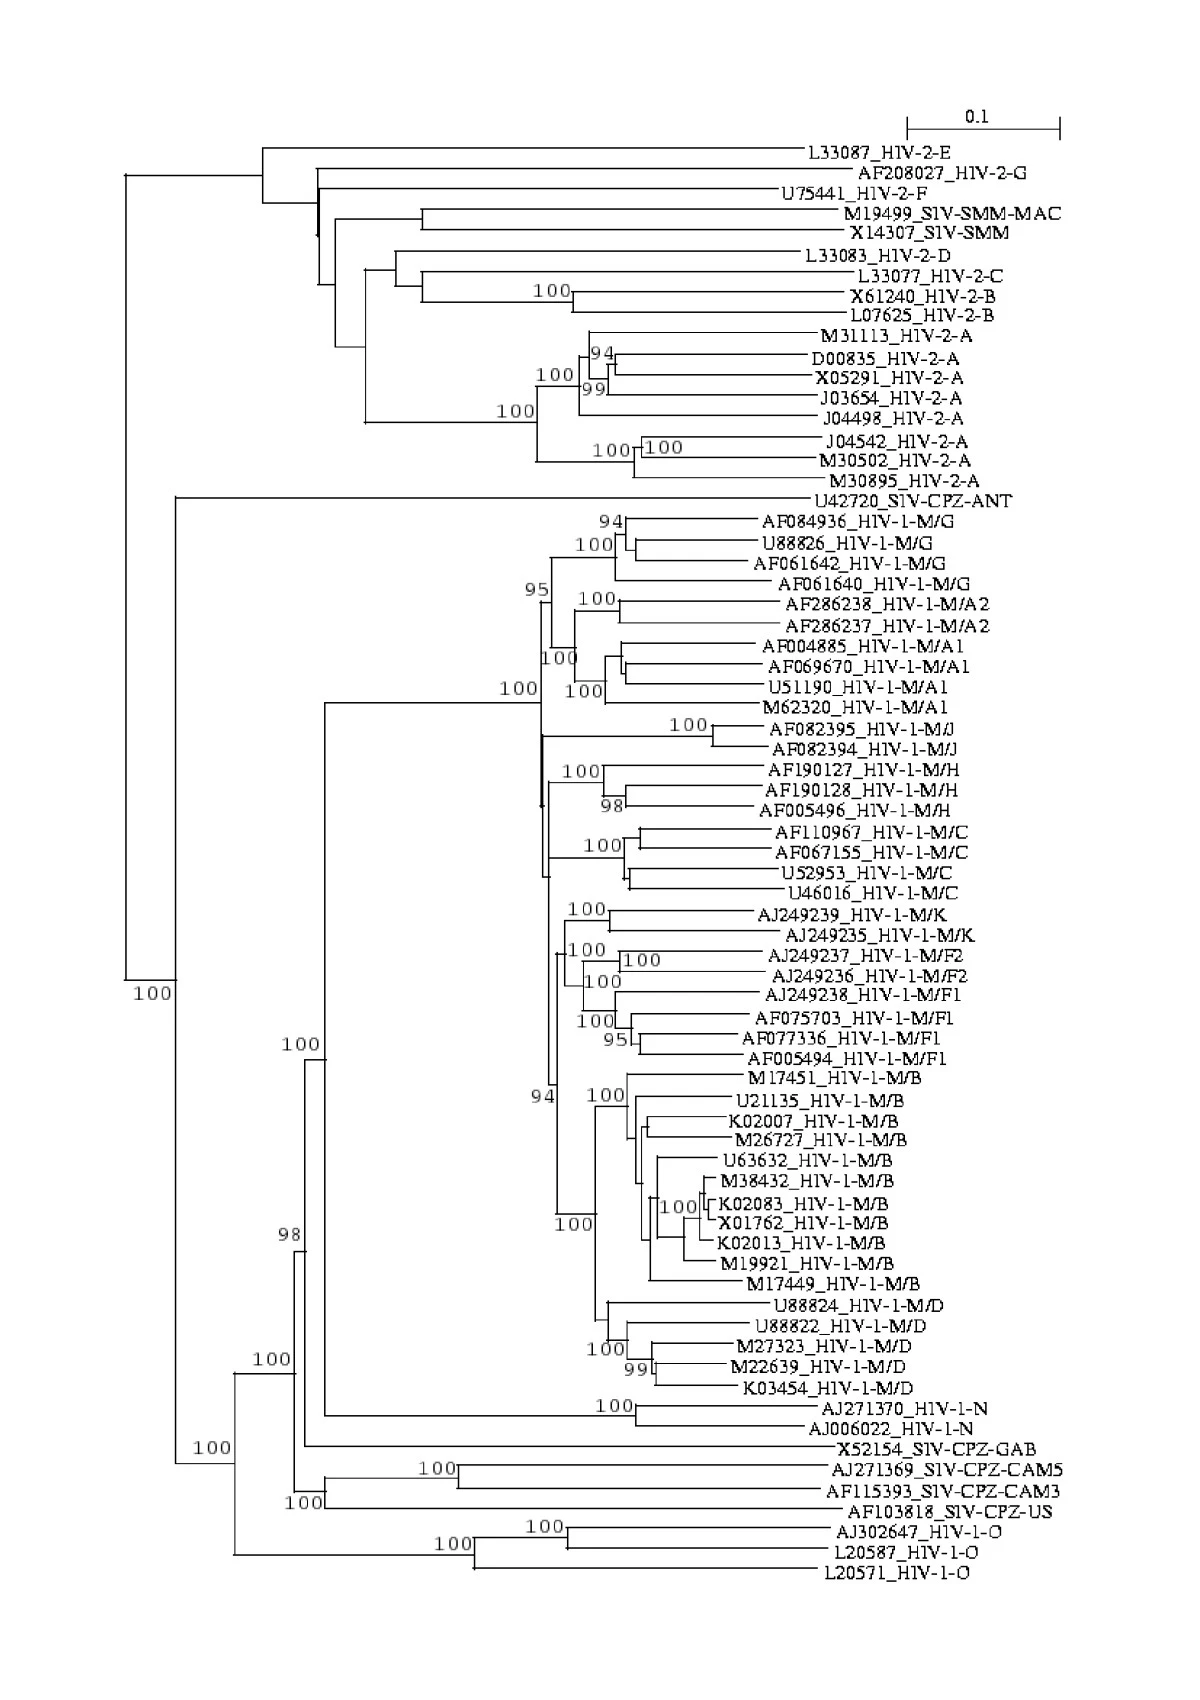
\includegraphics[width=\textwidth]{../data/Tree visualization/original_66_tree.png}
    \caption{Original tree obtained from the dissimilarity matrix of the sequences of the original article, with $N = 15$ - accesible in the repository at \texttt{data/Tree  visualization/original\_66\_tree.png}}
    \label{fig:original_tree66}
\end{figure}

\begin{figure}[H]
    \centering
    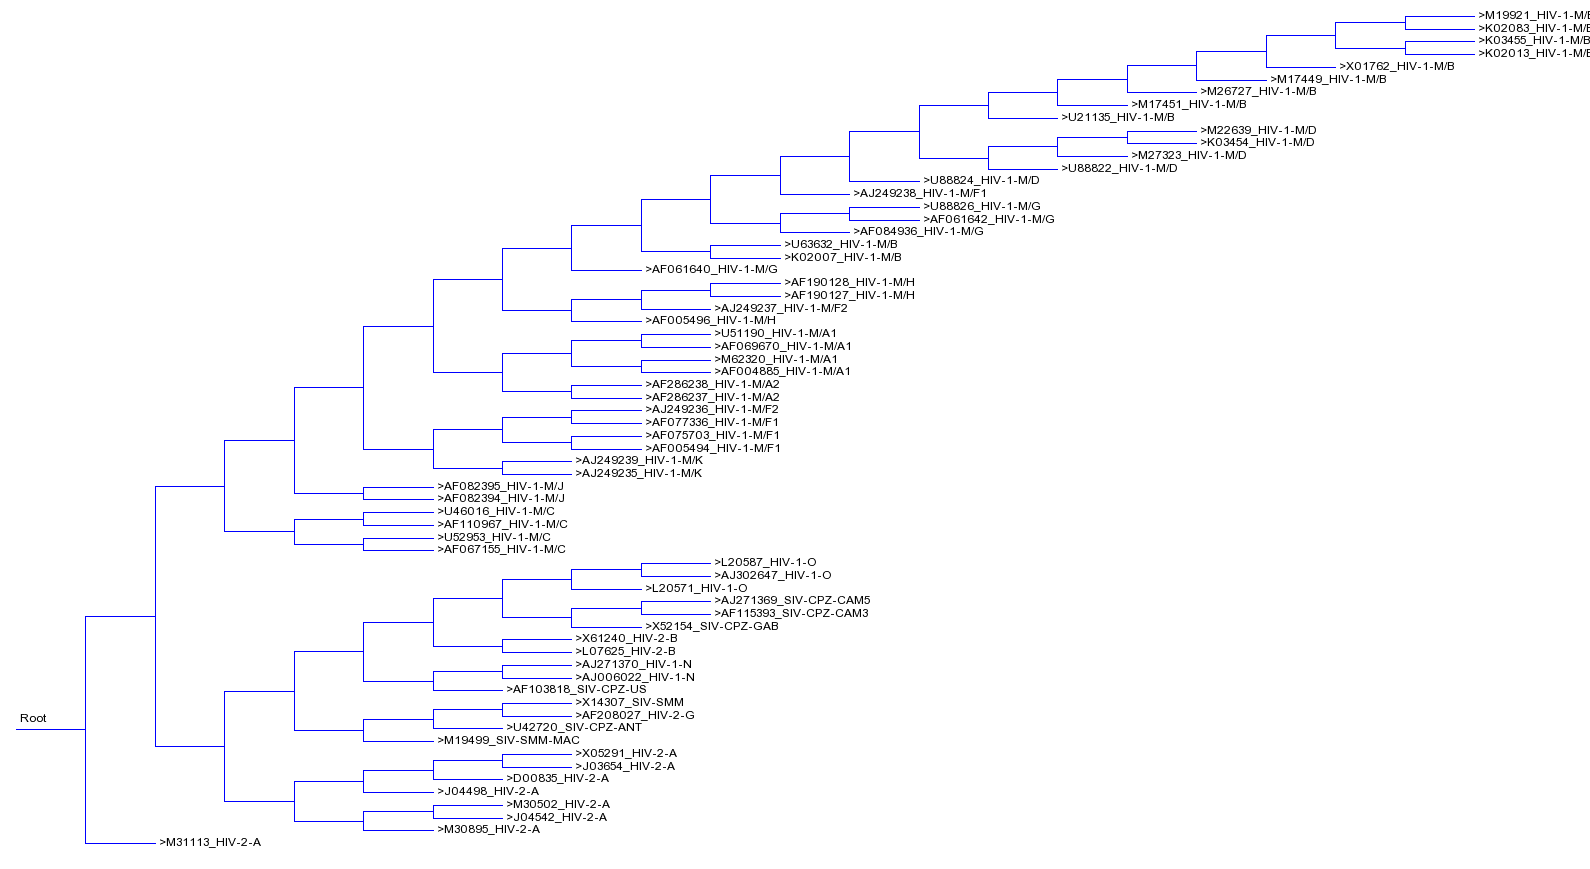
\includegraphics[width=.95\textheight, angle=90]{../data/Tree visualization/66_tree.png}
    \caption{Tree obtained from the dissimilarity matrix of the sequences of the original article, with $N = 15$ - accesible in the repository at \texttt{data/Tree  visualization/66\_tree.png}}
    \label{fig:tree66}
\end{figure}

\begin{figure}[H]
    \centering
    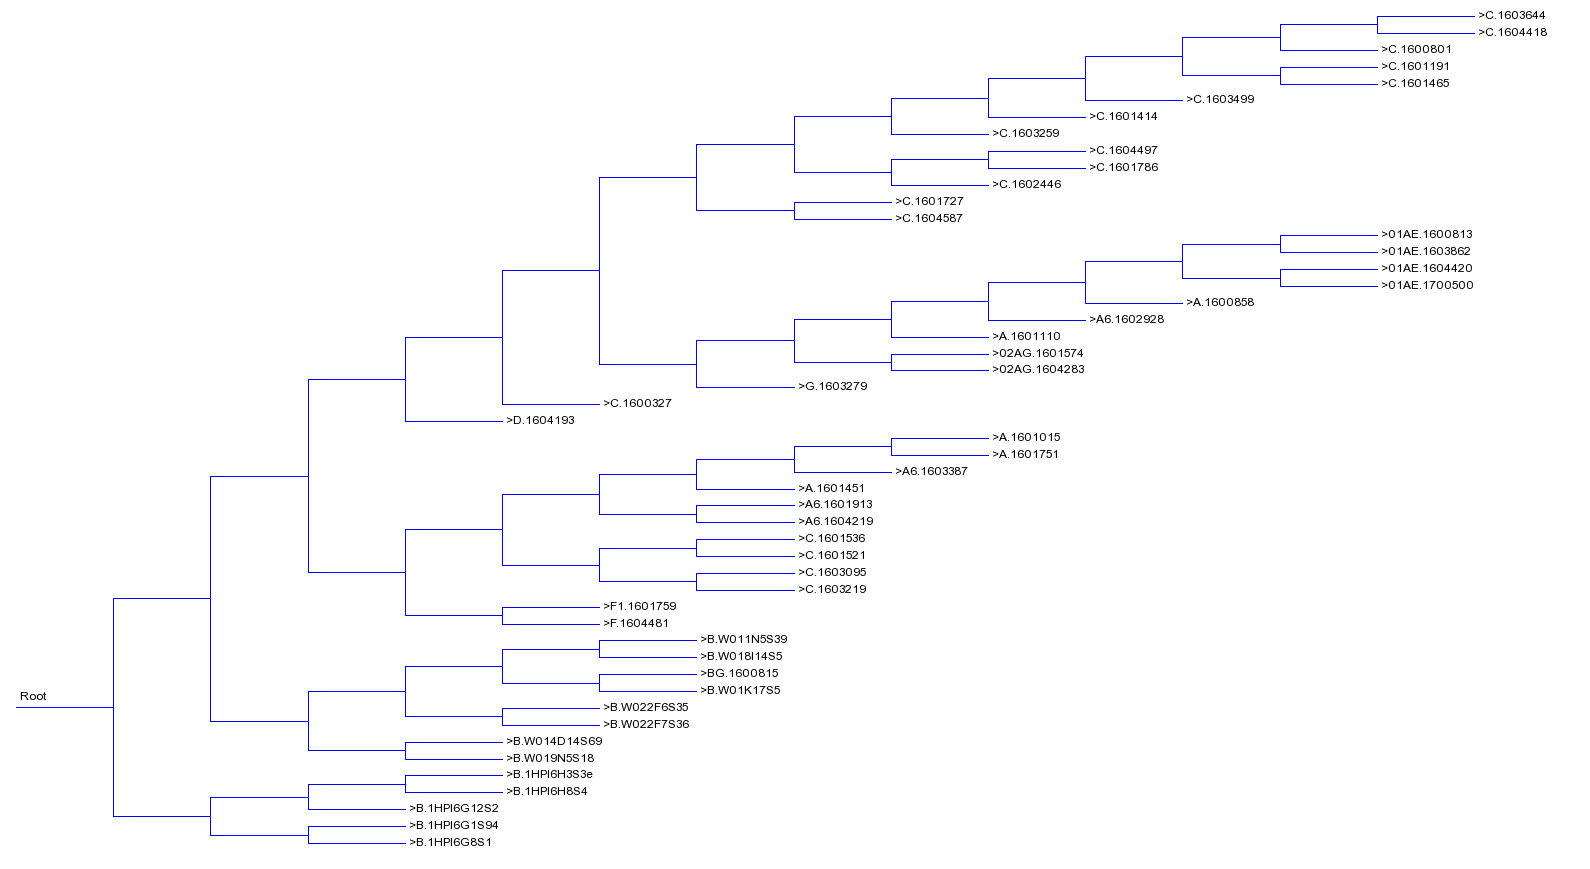
\includegraphics[width=.95\textheight, angle=90]{../data/Tree visualization/50_tree.png}
    \caption{Tree obtained from the dissimilarity matrix of the 50 sequences from Germany, with $N = 15$ - accesible in the repository at \texttt{data/Tree  visualization/50\_tree.png}}
    \label{fig:tree50}
\end{figure}


\end{document}